
\subsubsection{ALExa} 


\paragraph{Overview} 

The ALExa project ({\sl Accelerated Libraries for
Exascale})
focuses on preparing the DTK and Tasmanian libraries for
exascale platforms and integrating these libraries into ECP
applications.  These libraries deliver capabilities
identified as needs of ECP applications: (1) the ability to
transfer computed solutions between grids with differing
layouts on parallel accelerated architectures,
enabling simulation projects such as ExaAM and ExaSMR to
seamlessly combine results from different computational
grids to perform their required simulations (DTK); and (2) the
ability to construct surrogate models with low memory
footprint, low cost and optimal computational throughput, to
enable the use of methods for optimization and uncertainty
quantification for large scale engineering problems, as well
efficient multi-physics simulations in projects such as
ExaStar (Tasmanian).

These capabilities
are being developed through ongoing interactions with our
ECP application project collaborators to ensure they will
satisfy requirements of these customers.  The libraries in
turn take advantage of other ECP/SW capabilities currently in
development, including Trilinos, Kokkos and SLATE.  The
final outcome of the ECP project will be a set of
libraries deployed to facilities
and also made broadly available as part of the xSDK4ECP
project.

{\bf DTK} (Data Transfer Kit)
{\it Purpose:}
Transfers computed solutions between grids with differing
layouts on parallel accelerated architectures.
{\it Significance:} Coupled applications frequently have
different grids with different parallel distributions; DTK
is able to transfer solution values between these grids
efficiently and accurately.
{\it Mesh-free interpolation capabililities:}
multivariate data interpolation between point clouds;
compactly supported radial basis functions;
nearest-neighbor and moving least square implementations;
common applications include conjugate heat transfer,
fluid structure interaction, and mesh deformation.
{\it Performace portable search capabilities:}
threaded and GPU implementations of spatial tree
construction;
threaded and GPU implementations of various spatial tree
queries;
MPI front-end for coordinating distributed spatial searches
between sets of geometric objects with different
decompositions;
communication plan generation based on spatial search
results.
{\it URL:}
https://github.com/ORNL-CEES/DataTransferKit

{\bf Tasmanian} (Toolkit for Adaptive Stochastic Modeling
and Non-Intrusive Approximation)
{\it Purpose:} Constructs surrogate models for high
dimensional problems to help solve large scale engineering
and multiphysics problems
{\it Significance:}
Applications may require reduced representations of higher
dimensional data, for example, to optimize storage of high
dimensional tabular data or optimally perform UQ
calculations.  In addition, Tasmanian offers capabilities in
inverse problems, e.g., calibration and inference.
{\it Sparse grids capabilities:}
surrogate modeling and design of experiments (adaptive
multi-dimensional interpolation);
reduced (lossy) representation of tabulated scientific data;
high dimensional numerical quadrature;
data mining and manifold learning.
{\it DiffeRential Evolution Adaptive Metropolis (DREAM)
capabilities:}
Bayesian inference;
parameter estimation/calibration;
model validation.
global optimization and optimization under uncertainty.
{\it URL:}
http://tasmanian.ornl.gov

\paragraph{Key Challenges}

\indent

{\bf DTK:}
The general case of transferring data between grids of
unrelated applications requires an all-to-all
communication.
This is increasingly challenging as communication
to computation ratios are decreasing on successive HPC
systems.
Furthermore, the gridcell search procedures to locate
interpolation points require tree search methods
difficult to optimize on modern accelerated
architectures due to vector lane or thread divergence.
Also, maintaining high accuracy for the transfer requires
careful attention to the mathematical properties of the
interpolation methods and is highly application-specific.
Unlike other, ``black box'' libraries,
grid transfer methods may require close collaboration
with application partners to understand customer
requirements
(accuracy and conservation law requirements,
distribution of grids, location and layout of grid data in
memory hierarchy, etc.)

{\bf Tasmanian:}
Sparse grid methods require dense linear algebra operations
with matrix sizes that may be large.
These operations must be well-optimized for the target
architectures, including accelerated nodes.
Uncertainty quantification methods can require many runs of
an application as input to forming a surrogate model,
and the runs may have very different runtimes,
creating a scheduling problem that must be solved in order
to maximize performance.

\paragraph{Solution Strategy}

\nobreak


\indent

{\bf DTK:}
State of the art mathematically rigorous methods are used in
DTK to preserve accuracy of interpolated solutions.
Algorithms are implemented in a C++ code base with extensive
unit testing on multiple platforms.
Trilinos packages are used to support interpolation methods.
Kokkos is used to achieve performance portability
across accelerated platforms.

{\bf Tasmanian:}
To support performance portability across platforms for
dense linear algebra operations, a collaboration with the
SLATE ECP project is underway to take advantage of the new
library software being developed.
A DAG scheduler will be implemented under the project to
enable optimal execution of multiple application instances
for UQ problems.

%----------------------------------------

\paragraph{Recent Progress}

\indent

{\bf DTK:}
Ongoing work with a growing list of ECP application partners
is continuing.
Extensive work has been done to define the Fortran, C and
C++ DTK interfaces to support partner projects.
A set of benchmark problems has been developed
to guide DTK method and code development.
Recent progress has been made to optimize the search methods
for modern-generation GPUs.

\begin{figure}[htb]
        \centering
        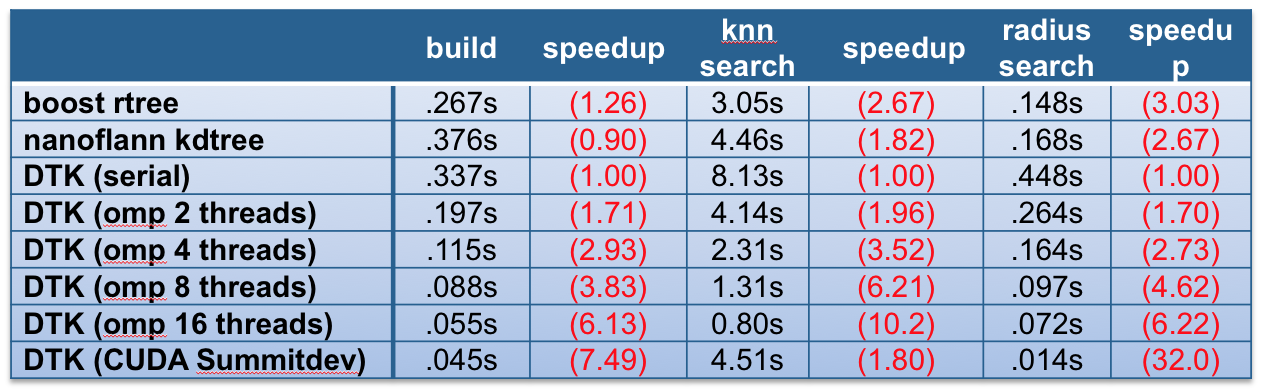
\includegraphics[width=4in]{projects/2.3.3-MathLibs/2.3.3.11-ALExa/dtk-gpu}
        \caption{\label{fig:dtk-gpu}DTK tree search, OpenMP and Summitdev GPU speedups}
\end{figure}

{\bf Tasmanian:}
The infrastructure of Tasmanian has been upgraded to support
the broader ECP focus of the work.
GPU acceleration of sparse grid surrogates has been
implemented.
Tasmanian recently enabled the ExaStar project
to reduce the size of a large-memory table of neutrino
opacities by 100X while still preserving accuracy.

\begin{figure}[htb]
        \centering
        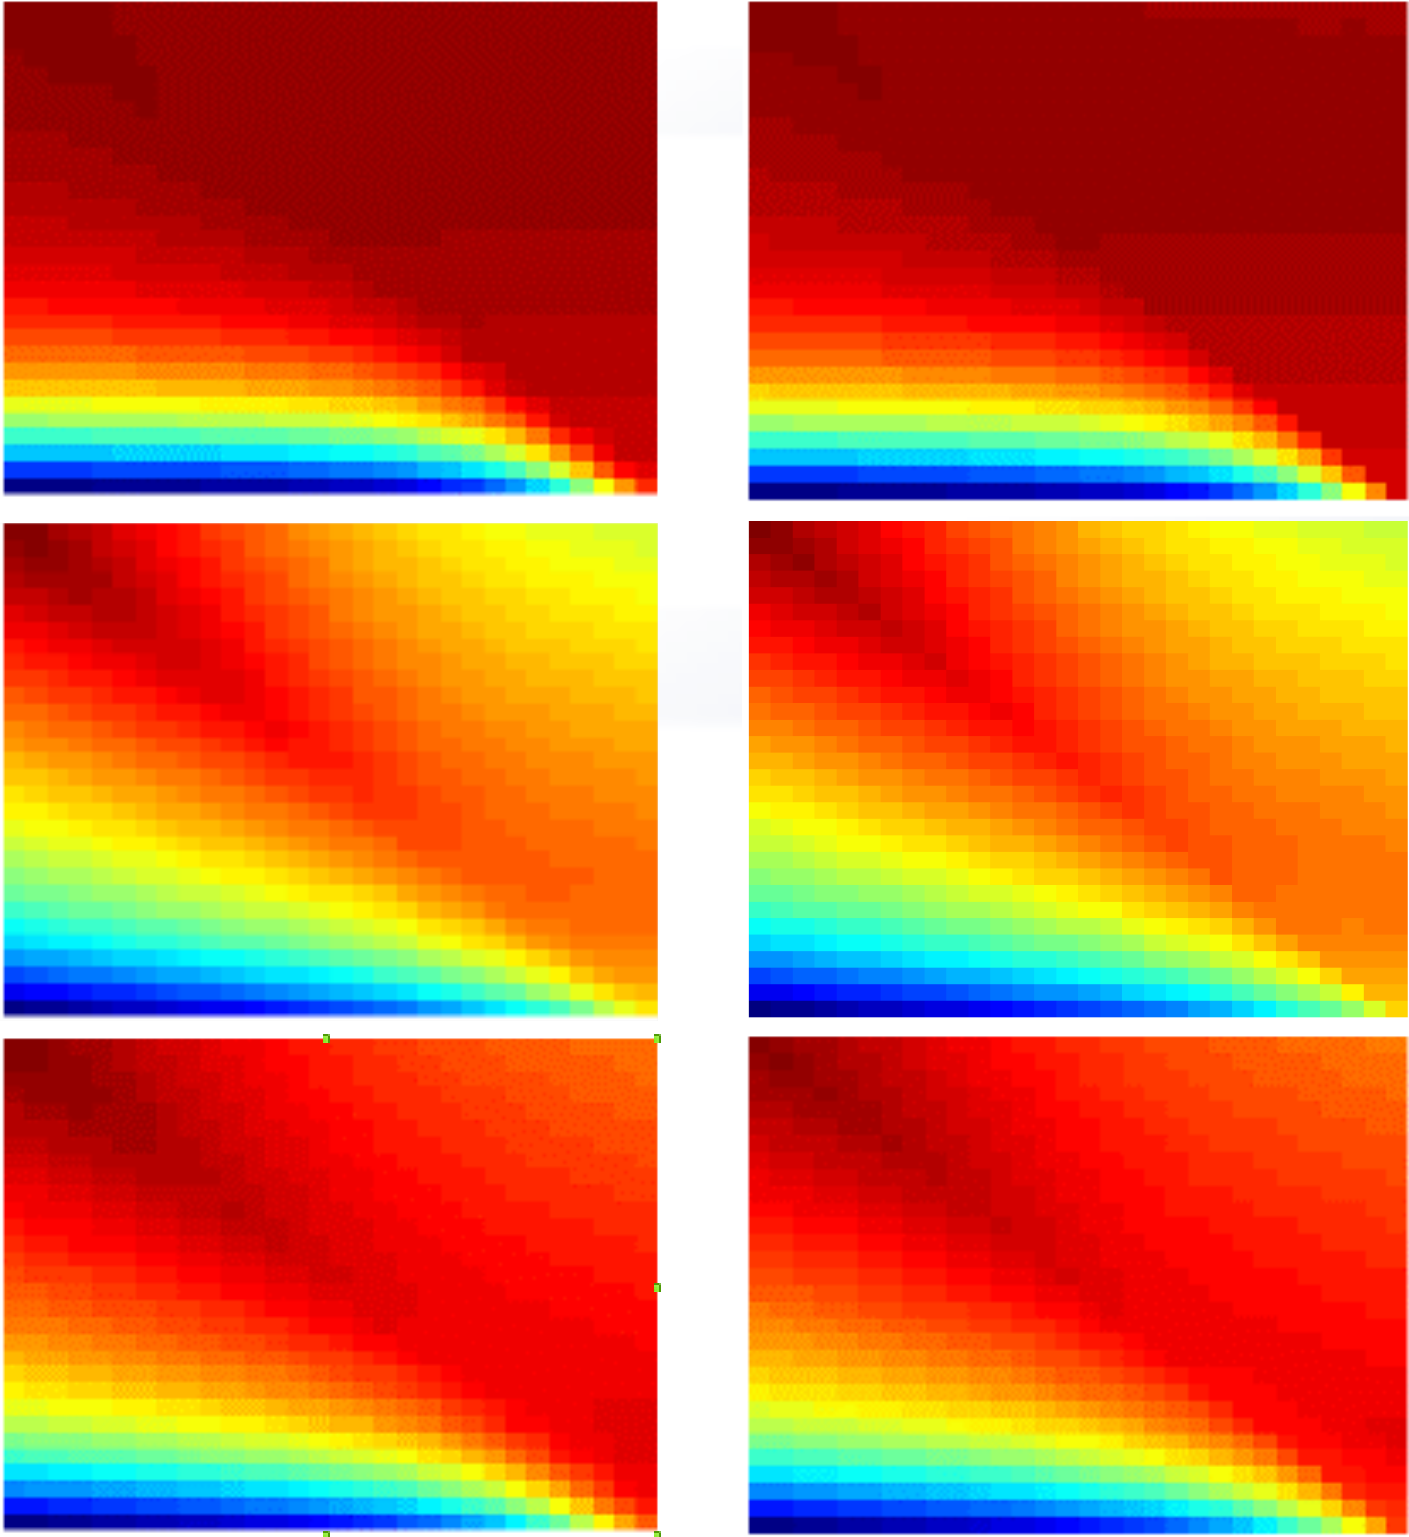
\includegraphics[width=2in]{projects/2.3.3-MathLibs/2.3.3.11-ALExa/tasmanian-gpu}
        \caption{\label{fig:tasmanian-gpu}Tasmanian speedup on Titan node using cuBLAS}
\end{figure}

%----------------------------------------

\paragraph{Next Steps}

\indent

{\bf DTK:}
A major focus for the near future is to optimize performance
for the targeted architectures using the developed benchmark
cases.
This will be followed by work on a showcase problem to
demonstrate performance.

{\bf Tasmanian:}
Work will continue to integrate the SLATE dense linear
algebra capabilities into Tasmanian to enable high
performance and performance portability.
Asynchronous sampling using DAG methods will be implemented
for the sparse grid methods.

%----------------------------------------

